\documentclass{../py-lecture}

\begin{document}

\begin{frame}
  \titlepage{}
\end{frame}
\begin{frame}
  \frametitle{Outline}
  \tableofcontents{}
\end{frame}

\section{Introduction}

%------------------------------------------------
\begin{frame}
\begin{columns}
	\begin{column}{10cm}
		\vspace{2cm}
		\begin{block}{
				\centering\textcolor{darkgray}{What is python...}}
				Python is a high-level, interpreted, interactive and object-oriented scripting language. Python is designed to be highly readable..
		\end{block}
	\end{column}
\end{columns}
\vspace{.75cm}
\hspace*{8.5cm}
\includegraphics[width=3cm]{img/python.jpeg}
\end{frame}

%------------------------------------------------
\begin{frame}
	\frametitle{Environment}
	\hspace*{1.5cm}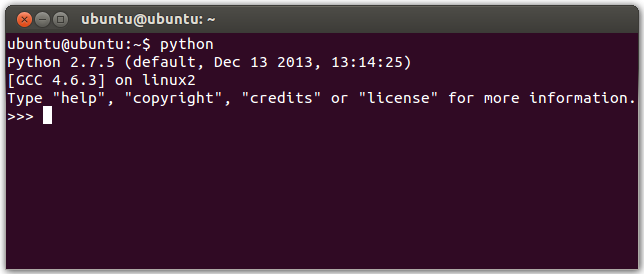
\includegraphics[width=10cm]{img/python-console-linux.png}
\end{frame}

\end{document}
